% File: paper.tex 
%  Cre: 2013-09-12 
%  $Id: paper.tex 4261 2015-01-27 23:49:04Z jhennawi $ 

\documentclass[iop]{emulateapj}
\bibliographystyle{apj}
\usepackage{amsmath} 
\usepackage{aas_macros,amssymb}
\usepackage{natbib,graphicx,layouts}
\usepackage{color,hyperref}
\usepackage{bm}
\definecolor{linkcolor}{rgb}{0,0,0.5}
\definecolor{notecolor}{rgb}{0.8,0,0}
\hypersetup{colorlinks=true,linkcolor=linkcolor,citecolor=linkcolor,
  filecolor=linkcolor,urlcolor=linkcolor}
\usepackage{tikz}
\usetikzlibrary{arrows,decorations.pathmorphing}

\shorttitle{Pressure smoothing in nonlinear IGM}
\shortauthors{Kulkarni et al.}

\begin{document}

\title{Flagging gravitational wave sources from radio jet morphology}
\author{Girish Kulkarni\altaffilmark{1} and
  Abraham Loeb\altaffilmark{2}}
\altaffiltext{1}{Institute of Astronomy, University of Cambridge,
  Madingley Road, Cambridge CB3 0HA, UK;
  \email{kulkarni@ast.cam.ac.uk}}
\altaffiltext{2}{Harvard}

\begin{abstract}
Apart from a stochastic gravitational wave (GW) background, LISA will
also be able to detect GW emission from binary black holes. The number
of such binary sources depends on the major merger rates of gas-rich
galaxies and subsequent evolution of their central black holes.  The
latter of these is uncertain.  Therefore, an alternate method of
flagging GW sources is useful.  Here we show that if one of the binary
BHs is accreting and has a jet, then the dynamical evolution of the
binary is imprinted on the jet morphology.  Using this dependance, it
is possible to flag binary BHs that are entering their GW inspiral
phase in the present epoch.  We further show that this relationship
between the binary dynamics and the jet morphology has two other
applications: (1) at large binary separations the Mpc-scale jet
morphology can probe the acts as a probe of the pc-scale gas supply to
the binary, and (2) at smaller separations the jet morphology acts as
a test of GR.
\end{abstract}

\keywords{cosmology: IGM} 

\section{Introduction}
\label{sec:intro}

Consider two black holes with masses $M_1$ and $M_2$ in a circular
orbit of radius $a$ around each other \citep{2010PhRvD..81d7503L}.
Let $M_1=M_2$ (assume equal masses for simplicity).  The orbital speed
of each black hole is given by
\begin{equation}
  v_\mathrm{orb} = \frac{1}{2}\left(\frac{GM}{a}\right)^{1/2} = 5.8\times 10^3\, \mathrm{km~s}^{-1}M_8^{1/2}a_{16}^{-1/2},
  \label{eqn:vorb}
\end{equation}
where $a_{16}\equiv a/10^{16}$ cm and $M_8\equiv M/10^8$
M$_\odot$. Now imagine a jet coming out of one of the BHs at an angle
$\chi$ to the direction of the orbital angular momentum.  Then because
of the orbital motion, the jet will sweep out a cone.  This is shown
in Figure \ref{fig:BH_orbit}.  The half opening angle of the cone is
given by
\begin{equation}
  \sin\psi = \frac{v_\mathrm{orb}\cos\chi}{v_\mathrm{jet}},
\end{equation}
where $v_\mathrm{jet}$ is the ballistic speed of the jet.  Figure
\ref{fig:jet} shows how this looks.

For observable predictions we have to project this in observer plane.
Let the angle between the jet direction and the observer line of sight
be $i$.  Then
\begin{equation}
  \psi^\mathrm{obs}\approx\frac{\psi}{\sin i}.
\end{equation}

\section{Jet structure when binary enters GW-induced inspiral}

Now when the binary is at the separation at which gravitational
wave-induced inspiral begins, it has a velocity given by Equation (5)
of your 2009 paper:
\begin{equation}
  v_\mathrm{orb} = 3.6\times 10^3\, \mathrm{km~s}^{-1}(\dot{\mathcal{M}}M_8)^{1/8},
  \label{eqn:v}
\end{equation}
where all symbols on the right hand side have the same meaning as in
your paper.  The separation between the two black at this instant is
given by Equation (7) of your paper:
\begin{equation}
  a = 8.3\times 10^{-3}\, \mathrm{pc}\, M_8^{3/4}\dot{\mathcal{M}}^{-1/4}.
\end{equation}
This gives
\begin{equation}
  \psi^\mathrm{obs}=2.42^\circ \left(\frac{v_\mathrm{jet}}{0.95 c}\right)^{-1}\cos\left(\frac{\chi}{30^{\circ}}\right)\left[\sin\left(\frac{i}{15^{\circ}}\right)\right]^{-1},
\end{equation}
This value in itself is probably not very interesting as it depends on
$v_\mathrm{jet}$ and $\chi$, but it gets interesting when we consider
the evolution of $\psi^\mathrm{obs}$ below.

\begin{figure}
  \begin{center}
    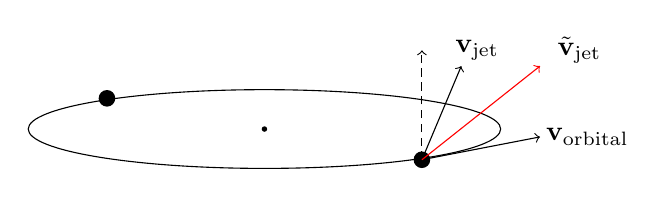
\begin{tikzpicture}
      \draw (0,0) ellipse (3 and 0.5);
      \fill[black] (0,0) circle (1pt);
      %\draw [->,densely dashed] (0,0) -- (0,2.0);
      \fill[black] (2,-0.39) circle (3pt);
      \fill[black] (-2,0.39) circle (3pt);
      \draw [->] (2,-0.39) -- (3.5,-0.1);
      \draw [->,densely dashed] (2,-0.39) -- (2,1.0);
      \draw [->] (2,-0.39) -- (2.5,0.8);
      \draw [->,red] (2,-0.39) -- (3.5,0.8);
      \draw (4.1,-0.1) node {${\mathbf{v}}_\mathrm{orbital}$};
      \draw (2.7,1.0) node {${\mathbf{v}}_\mathrm{jet}$};
      \draw (4.0,1.0) node {$\tilde{\mathbf{v}}_\mathrm{jet}$};
    \end{tikzpicture}
  \end{center}
  \caption{Jet and orbital configuration. The effect of
    $\mathbf{v}_\mathrm{orbital}$ is to precess the jet as the BH
    moves along the orbit. Note that
    $\tilde{\mathbf{v}}_\mathrm{jet}={\mathbf{v}}_\mathrm{orbital}+{\mathbf{v}}_\mathrm{jet}$.}
  \label{fig:BH_orbit}
\end{figure}

\section{Evolution of jet structure}

Binary separation, jet velocity, and the two angles, tell us about the
instantaneous configuration of the jet.  (Recall that we are only
considering an equal mass binary.)  The jet evolution is governed by
the dynamical evolution of the binary separation.  During the
gas-dominated phase, this is given by
\begin{equation}
\frac{a}{\dot a} = \mu/\dot M = 1.1\times 10^7\, \mathrm{yr}\,\dot{\mathcal{M}}^{-1}.   
\end{equation}
This increases by two orders of magnitude during the GW phase to
\begin{equation}
\frac{a}{\dot a} = \frac{5}{256}\frac{c^5a^4}{G^3M^2\mu}=2.53\times 10^5\,\mathrm{yr}\,\frac{a_{16}^4}{M_8^3}.
\end{equation}
From Equation (\ref{eqn:vorb}), the orbital velocity of each BH evolves as
\begin{equation}
  \frac{\dot v_\mathrm{orb}}{v_\mathrm{orb}} = -\frac{1}{2}\frac{\dot a}{a}.
\end{equation}
which gives the evolution of the opening angle of the cone as 
\begin{equation}
  \dot\psi^\mathrm{obs}=\dot\psi = -\frac{1}{2\cot\psi}\frac{\dot a}{a}.
\end{equation}
This can be solved analytically to get
\begin{equation}
  \sin\psi = \sin\psi_0\left(\frac{a_0}{a}\right),
\end{equation}
where $\psi_0$ and $a_0$ are the initial values. Thus as the binary
continues to shrink the BH orbital velocity grows and the opening
angle of the conical jet increases (cone gets wider and wider).  The
rate at which this happens tells everything about the binary's
dynamical evolution.

Figures \ref{fig:a_gw} show this evolution for the numbers assumed
above.

\section{Use jets to flag GW binaries}

Figure \ref{fig:a_gas} shows the evolution of the binary when it is in
the gas accretion phase.  We have chosen steady gas accretion with
$\dot{\mathcal{M}}=1$ here for simplicity.  Note that the starting
separation here is about 100 pc. 

What we find is that in the beginning the binary orbital period is
about $10^7$ yr. So the jet will show no signs of precision at this
point.  However as the binary separation reduces to about 10 pc, the
period reduces to $\sim 100$ yr and the jet will start showing
precision.  At this point the time scale for binary merger is $\sim
10^7$ yr.

In other words \emph{since the gas accretion time scale is of the
  order of the typical jet lifetime} the jet structure will show a
transition from a straight jet to a precessing jet at a separation of
\begin{equation}
  v_\mathrm{apparant}\left(\frac{t_0}{10^7}\right).
\end{equation}
from the binary.  \textbf{[Convert this to arcseconds on the sky.]}
The location at which the jet morphology shows this precision and the
opening angle evolution give a direct constraint on the epoch of
graviational wave emission of the binary.

Thus the new insight here is that the signature of the jet precision
due to GW-inspiral is observationally accessible. 

\section{Jet morphology as probe of GR}

Variability of lensed quasars constraints the size of accretion disks
to about $10^{15}$ cm ($\sim 10^{-3}$ pc) \citep{2010ApJ...712.1129M}.
This is smaller than the $a_\mathrm{GW}$ by a factor of less than 10.

This means that the GW-induced precision will be visible in the jet
precision for a very short distance near the source before the
accretion disk is disrupted.

Last plots in this note show some example jets.  In all these plots
$\psi$ is the half-opening angle of the conical jet, and $i$ is the
angle between the jet and the line of sight.

A rough argument about observability: For our example, the period is
0.1 yr at $t = 63967.3816055$ yr.  We can assume that the chirp begins
at $t = 10^4$ yr when period is $\sim 2$ yr.  So the total duration of
the chirp is $5.3\times 10^4$ yr.

A 2 yr period gives $\sim 1$ milli-arcsec wiggles in the jet.  So the
idea is that the wiggles will change from milli-arcsec to micro-arcsec
over $\sim 10^5$ yr.  That is over a length scale of $\sim 30$ kpc.

Now the question is: how big an angle would a 30 kpc jet subtend on
the sky in arcsecs?

Let us assume $z = 0.302$ which is the redshift of 1928+738 jet that
Roos (1993) have studied.  At this redshift 30 kpc will subtend about
6.748195445702 arcsec.

So we are talking about mciro- to milli-arcssec scale wiggles in tens
of arcsec scale jets.  Jets are routinely seen over hundreds of
arcsec.



\section{Conclusion}

From Figures \ref{fig:a_gw} we can make these four points:

\begin{itemize}
\item From the jet structure, we can tell how long until the binary enters GW-induced inspiral.
\item In particular, we can flag binaries that are entering GW-inspiral now.
\item We could locate binaries that are now in GW inspiral phase but
  have helical jet structures that are impossible to resolve.
\item From the above jet structure, we get an idea of the history of gas inflow on the binary.
\end{itemize}

There will also probably be some spectral evolution along the jet.
This spectral evolution will act as a cross check on the evolution
deduced from the jet morphology.  An important advantage of this
technique is that it allows us to locate binaries that may be
impossible to locate even with VLBI.

\begin{figure}
  \begin{center}
    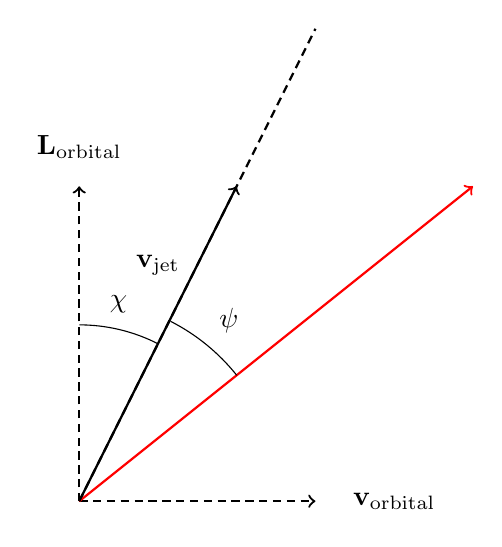
\begin{tikzpicture}
      \draw [->,densely dashed,thick] (0,0) -- (3.0,0);
      \draw [->,densely dashed,thick] (0,0) -- (0,4.0);
      \draw [->,thick] (0,0) -- (2.0,4.0);
      \draw [->,thick,red] (0,0) -- (5.0,4.0);
      \draw (1.0,2.0) arc (63:90:2.2);
      \draw (2.0,1.6) arc (38.6:63:2.56);
      \draw (0.5,2.5) node {$\chi$};
      \draw (1.90,2.3) node {$\psi$};
      \draw [densely dashed,thick] (0,0) -- (3.0,6.0);
      \draw (0.0,4.5) node {$\mathbf{L}_\mathrm{orbital}$};
      \draw (4.0,0.0) node {$\mathbf{v}_\mathrm{orbital}$};
      \draw (1.0,3.0) node {$\mathbf{v}_\mathrm{jet}$};
    \end{tikzpicture}
  \end{center}
  \caption{The orbital velocity $\mathbf{v}_\mathrm{orbital}$
    introduces the jet precision angle $\psi$.  Without the orbital
    motion, $\psi=0$ and the jet traces a cylindrical surface.  With
    the orbital motion, as the BH moves along its circular orbit, the
    red vector oscillates around the solid black vector and produces a
    conical surface with $\psi$ as its half-opening angle.  Note that
    $v_\mathrm{orbital}$ is exagerated here.  In practice,
    $v_\mathrm{orbital}\ll v_\mathrm{jet}\sim c$.  This figure then
    shows that
    $\sin{\psi}\sim\tan{\psi}=v_\mathrm{orbital}\cos{\chi}/v_\mathrm{jet}$.}
  \label{fig:jet}
\end{figure}

\begin{figure*}
\begin{center}
  \begin{tabular}{ccc}
    \includegraphics*[width=2.2in]{a_gw.pdf} &
    \includegraphics*[width=2.2in]{v_orb.pdf} &
    \includegraphics*[width=2.2in]{psi.pdf}
  \end{tabular}
\end{center}
\caption{Evolution of the binary separation.  Time $t$ is time since the gravitational wave induced phase began.}
\label{fig:a_gw}
\end{figure*}

\begin{figure*}
\begin{center}
  \begin{tabular}{ccc}
    \includegraphics*[width=2.2in]{a_gas.pdf} &
    \includegraphics*[width=2.2in]{v_orb_gas.pdf} &
    \includegraphics*[width=2.2in]{psi_gas.pdf}
  \end{tabular}
\end{center}
\caption{Evolution of the binary separation.  Time $t$ is time since the gravitational wave induced phase began.}
\label{fig:a_gas}
\end{figure*}

%% \begin{figure}
%%   \begin{center}
%%     \includegraphics*[width=\columnwidth]{a_gw.pdf}
%%   \end{center}
%%   \caption{Evolution of the binary separation.  Time $t$ is time since
%%     the gravitational wave induced phase began.}
%%   \label{fig:a_gw}
%% \end{figure}

%% \begin{figure}
%%   \begin{center}
%%     \includegraphics*[width=\columnwidth]{v_orb.pdf}
%%   \end{center}
%%   \caption{Evolution of the orbital velocity}
%%   \label{fig:v_orb}
%% \end{figure}

%% \begin{figure}
%%   \begin{center}
%%     \includegraphics*[width=\columnwidth]{psi.pdf}
%%   \end{center}
%%   \caption{Evolution of the intrinsic half-opening angle of the
%%     conical jet.  it is important to note that the jet lifetime is
%%     about $10^7$ yr.}
%%   \label{fig:psi}
%% \end{figure}

\pagebreak
\pagebreak

\clearpage

\begin{figure}
  \begin{center}
    \includegraphics[width=\columnwidth]{jet_i10_psi20.pdf}
  \end{center}
  \caption{$i=10^\circ$, $\psi=20^\circ$, $\beta=0.90$}
\end{figure}

\begin{figure}
  \begin{center}
    \includegraphics[width=\columnwidth]{jet_i40_psi20.pdf}
  \end{center}
  \caption{$i=40^\circ$, $\psi=20^\circ$, $\beta=0.90$}
\end{figure}

\begin{figure}
  \begin{center}
    \includegraphics[width=\columnwidth]{jet_i80_psi20.pdf}
  \end{center}
  \caption{$i=80^\circ$, $\psi=20^\circ$, $\beta=0.90$}
\end{figure}

\begin{figure}
  \begin{center}
    \includegraphics[width=\columnwidth]{jet_i40_psi40.pdf}
  \end{center}
  \caption{$i=40^\circ$, $\psi=40^\circ$, $\beta=0.90$}
\end{figure}

\clearpage

\begin{figure*}
\begin{center}
  \begin{tabular}{ccc}
    \includegraphics*[width=2.2in]{jet_i40_psi20_beta_0_90.pdf} &
    \includegraphics*[width=2.2in]{jet_i40_psi20_beta_0_80.pdf} &
    \includegraphics*[width=2.2in]{jet_i40_psi20_beta_0_40.pdf}
  \end{tabular}
\end{center}
\caption{Jet structure in the source frame. $\beta=0.9, 0.8, 0.4$ from left to right.}
\label{fig:srcframe}
\end{figure*}

\begin{figure*}
\begin{center}
  \begin{tabular}{ccc}
    \includegraphics*[width=2.2in]{jet_i40_psi20_beta_0_90_obs.pdf} &
    \includegraphics*[width=2.2in]{jet_i40_psi20_beta_0_80_obs.pdf} &
    \includegraphics*[width=2.2in]{jet_i40_psi20_beta_0_40_obs.pdf}
  \end{tabular}
\end{center}
\caption{Jet structure in the observer frame. $\beta=0.9, 0.8, 0.4$ from left to right.}
\label{fig:obsframe}
\end{figure*}

\begin{figure*}
\begin{center}
  \begin{tabular}{ccc}
    \includegraphics*[width=2.2in]{jet_i40_psi20_beta_0_90_ang.pdf} &
    \includegraphics*[width=2.2in]{jet_i40_psi20_beta_0_80_ang.pdf} &
    \includegraphics*[width=2.2in]{jet_i40_psi20_beta_0_40_ang.pdf}
  \end{tabular}
\end{center}
\caption{Jet structure in angular coordinates. $\beta=0.9, 0.8, 0.4$ from left to right.}
\label{fig:ang}
\end{figure*}

\begin{figure*}
\begin{center}
  \begin{tabular}{ccc}
    \includegraphics*[width=2.2in]{jet_i40_psi20_beta0_90_full.pdf} &
    \includegraphics*[width=2.2in]{jet_i40_psi20_beta0_90_zoom1.pdf} &
    \includegraphics*[width=2.2in]{jet_i40_psi20_beta0_90_zoom2.pdf}
  \end{tabular}
\end{center}
\caption{Jet morphology without accounting for opening angle
    evolution}
\label{fig:jet_nopsi}
\end{figure*}

\begin{figure*}
\begin{center}
  \begin{tabular}{ccc}
    \includegraphics*[width=2.2in]{jet_i40_beta0_90_full.pdf} &
    \includegraphics*[width=2.2in]{jet_i40_beta0_90_zoom1.pdf} &
    \includegraphics*[width=2.2in]{jet_i40_beta0_90_zoom2.pdf}
  \end{tabular}
\end{center}
\caption{Jet morphology with opening angle evolution.}
\label{fig:jet_psi}
\end{figure*}

\bibliography{refs}
\end{document}


